\documentclass{IEEEtran}

\usepackage[activate={true,nocompatibility},final,tracking=true,kerning=true,spacing=true,factor=1100,stretch=10,shrink=10]{microtype}
\linespread{0.96}

\usepackage{amsmath}
\usepackage{bm}
\usepackage{amssymb}
\usepackage{algorithm}
\usepackage{algorithmic}
\usepackage{stfloats}

\ifCLASSINFOpdf
   \usepackage[pdftex]{graphicx}
\else
   \usepackage[dvips]{graphicx}
\fi

\ifCLASSOPTIONcompsoc
  \usepackage[caption=false,font=normalsize,labelfont=sf,textfont=sf]{subfig}
\else
  \usepackage[caption=false,font=footnotesize]{subfig}
\fi

\usepackage[style=ieee,maxbibnames=1,minbibnames=1,maxcitenames=1,mincitenames=1,backend=biber,defernumbers=false]{biblatex}
\addbibresource{./bibtex/bib/Biblio.bib}

\begin{document}
\title{Impact of Time-of-Flight on Respiratory Motion Modelling using Non-Attenuation-Corrected PET}

\author{Alexander~C.~Whitehead~(\IEEEmembership{Student~Member~IEEE}),
        Elise~C.~Emond~(\IEEEmembership{Student~Member~IEEE}),
        Nikos~Efthimiou~(\IEEEmembership{Member~IEEE}),
        Adeyemi~Akintonde~(\IEEEmembership{Student~Member~IEEE}),
        Brian~F.~Hutton~(\IEEEmembership{Senior~Member~IEEE}),
        Jamie~McClelland
        and~Kris~Thielemans~(\IEEEmembership{Senior~Member~IEEE})%
        
    \vspace{-0.5cm}

    \thanks{This research is supported by GE Healthcare, the NIHR UCLH Biomedical Research Centre and the EPSRC-funded UCL Centre for Doctoral Training in Medical Imaging (EP/L016478/1).}%
    \thanks{Elise~C.~Emond is supported by GlaxoSmithKline (BIDS3000030921).}%
    \thanks{Alexander~C.~Whitehead, Elise~C.~Emond, Brian~F.~Hutton and Kris~Thielemans are with the Institute of Nuclear Medicine, University College London, London, NW1~2BU, UK (contact: \texttt{alexander.whitehead.18@ucl.ac.uk}.}%
    \thanks{Nikos Efthimiou is with the PET Research Centre, Faculty of Health Sciences, University of Hull, Hull, HU6~7RX, UK}%
    \thanks{Adeyemi~Akintonde and Jamie~McClelland are with the Centre for Medical Image Computing, University College London, London, NW1~2BU, UK.}%
}

\maketitle
\vspace{-1cm}

\IEEEpeerreviewmaketitle
\vspace{-1cm}

\begin{abstract}
Respiratory motion reduces image quality in PET. Unless gated CT or MR data are available, motion correction relies on registration of the PET data. To avoid mis-registration due to attenuation mismatches, most existing methods rely on pair-wise registration of Non-Attenuation-Corrected (NAC) PET volumes. This is a challenging problem due to the low contrast and high noise of these volumes. This paper investigates the possibility of using motion models for respiratory motion correction in PET, and in particular whether incorporating Time-of-Flight (TOF) information increases the accuracy of the motion models derived from the NAC reconstructed images. XCAT phantom simulations are used for one bed position with a field of view including the base of the lungs and the diaphragm. A TOF resolution of 375ps is used. NAC images are reconstructed using OSEM and used as input for motion model estimation. Different motion models are compared using the original XCAT input volumes. The results indicate that TOF improves the accuracy of the motion model considerably.

\end{abstract}

\vspace{-0.4cm}

\section{Introduction}
\IEEEPARstart{R}{espiratory} motion causes artefacts and loss of resolution in the thoracic region in PET~\cite{Nehmeh2008}. Many methods have been proposed to correct for respiratory motion, usually involving registration between a reference volume and a set of volumes in different positions in the respiratory cycle obtained by gating~\cite{Oliveira2014}. However, such pair-wise registration is sensitive to noise. It also does not allow prediction of the respiratory state for data not used to estimate the motion, for instance, to be used for real time motion correction. Surrogate driven motion models attempt to overcome these deficiencies by relating the motion in the data to a surrogate signal~\cite{McClelland2013}. The model outputs a transformation or deformation field for every value of the surrogate signal. Motion models are calculated on a series of either time or gating based volumes.

The benefits of using attenuation correction for PET image registration are unclear. If images are reconstructed using a static attenuation map ($\mu$-map), then artefacts caused by the misalignment between the activity distribution and the $\mu$-map would hamper image registration. It could therefore be advantageous to estimate motion on Non-Attenuation-Corrected (NAC) images~\cite{WenjiaBai2011}. However, contrast may be too low to calculate an accurate motion model and artefacts associated with the mismatch between the acquisition and system model could also obscure the underlying motion. 

In the absence of Time-of-Flight (TOF), there is no information on the activity position along the Line-of-Response (LOR), therefore, NAC reconstruction will place the activity towards the surface of the body and along low-density LORs. In TOF, the time information constrains the activity position along the LOR changing the nature and extent of the artefacts associated with NAC. The volumes are different in their expectation not just their noise properties.

The aim of this work is to investigate whether TOF can sufficiently increase the contrast and lower the noise of NAC images to facilitate the calculation of accurate motion models.

\vspace{-0.2cm}

\section{Methods}
XCAT~\cite{Segars2010} was used to generate $6$ volumes over a linear $5$ second breathing cycle, with $1$ volume at full expiration at the beginning of the cycle and $1$ volume at full expiration at the end of the cycle and using settings for the extent of Anterior-Posterior (AP) and Inferior-Superior (IS) motion. Activity concentrations were derived from a static FDG patient scan. The field of view included the base of the lungs, diaphragm and the top of the liver with a $40$mm diameter spherical lesion placed in the right lung.

PET acquisitions were simulated using STIR~\cite{Thielemans2012,Efthimiou2018} through SIRF~\cite{Ovtchinnikov2017} to forward project the input data to sinograms using the geometry of a GE Discovery 710 and, where relevant, a TOF resolution of $375$ps similar to the GE Signa (using TOF mashing to reduce computation time resulting in $13$ TOF time bins of size $376.5$ps). Attenuation was included in the simulation using the relevant $\mu$-map generated by XCAT. Scatter and randoms were not taken into account in the simulation. Multiple noise realisations were generated to simulate an acquisition as if it had been gated into $6$ bins over an acquisition of $120$s, emulating a standard single bed position acquisition. Data were reconstructed without attenuation correction using OSEM with $9$ full iterations and $18$ subsets~\cite{Hudson1994}. 

3D B-splines were used to model spatial deformations with the corresponding warping operation denoted as $\mathbf{W}(\mathbf{\alpha}_t)$, with $\mathbf{\alpha}_t$ a vector with B-spline coefficients at time $t$. The breathing surrogate signal $\mathbf{s}$ contained $2$ components, the AP and SI motion signals used by the XCAT.  Following~\cite{McClelland2013} a direct correspondence motion model was used where the B-spline coefficients at time $t$ are expressed as a linear combination of the $2$ components of the surrogate, $s_{1,t}$ and $s_{2,t}$:

\begin{equation}
    \forall t \in [[1,n_t]],\quad \alpha_{k,t} := R_{1,k} s_{1,t} + R_{2,k} s_{2,t} + R_{3,k}
\end{equation}

\noindent where $\alpha_{k,t}$ is the 3D B-spline coefficient for node $k$ at time point $t$, and $R_{i,k}$ are the model parameters. 

NiftyRegResp was used to estimate the Respiratory-Correspondence-Model (RCM), which is the object that takes in a surrogate signal value and a volume and warps the volume based on the value of the surrogate signal object, of the motion models, using sum of squared differences as an objective function~\cite{McClelland2017}.

\vspace{-0.2cm}

\section{Results}
\begin{figure*}
    \vspace{-0.2cm}
    
    \centering
    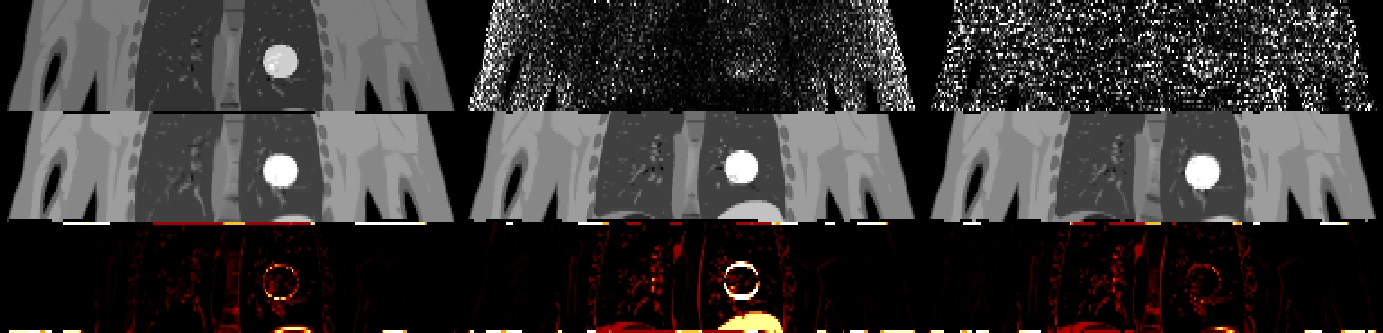
\includegraphics[width=0.9\linewidth]{figures/output.png}
    \caption{All volumes correspond to end-inhalation. First row from left to right: XCAT PET data, NAC nonTOF reconstructed data and NAC TOF reconstructed data. Second row: RCM applied to mean position XCAT data with RCM derived from XCAT PET data (left), NAC nonTOF (middle) and NAC TOF (right) volumes. Colour map ranges are consistent for all images on this row. The third row from left to right: The difference between the estimated volumes from the second row with the XCAT end-inhalation volume. Colour map ranges are consistent for all images on this row.}
    \label{fig:output}
    
    \vspace{-0.2cm}
\end{figure*}

\begin{table}
    \vspace{-0.2cm}
    
    \centering
    \small
    \caption{Comparison of the MSE between the ground truth data and the volumes estimated from the XCAT based RCM, the volumes estimated from the NAC nonTOF based RCM and the volumes estimated from the NAC TOF based RCM.}
    \begin{tabular}{||c|ccc||}
        \hline
            \textbf{MSE}    & \textbf{XCAT} & \textbf{nonTOF}   & \textbf{TOF}  \\
        \hline
            \textbf{$1$}    & $24707$       & $20020$           & $31370$       \\
            \textbf{$2$}    & $28595$       & $39309$           & $30445$       \\
            \textbf{$3$}    & $24242$       & $75570$           & $35417$       \\
            \textbf{$4$}    & $26127$       & $59310$           & $32519$       \\
            \textbf{$5$}    & $26459$       & $12951$           & $26120$       \\
            \textbf{$6$}    & $24707$       & $20020$           & $31370$       \\
        \hline
            \textbf{Mean}   & $26026$       & $41432$           & $31174$       \\
        \hline
    \end{tabular}
    \label{tab:mse}
    
    \vspace{-0.2cm}
\end{table}

\begin{figure}
    \vspace{-0.2cm}
    
    \centering
    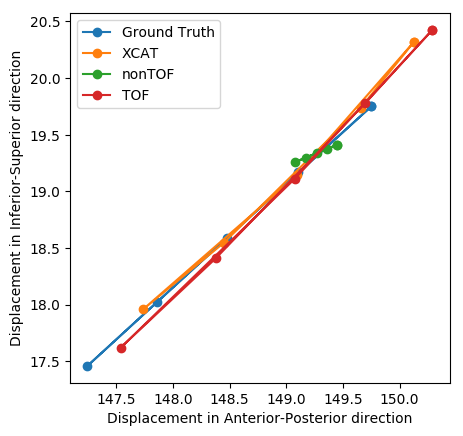
\includegraphics[width=0.7\linewidth]{figures/com_graph.png}
    \caption{The path of the Centre-of-Mass (COM) of the lesion. Horizontal (respectively vertical) axis corresponds to motion in the AP (respectively IS) direction over the $6$ gates. Different curves denote COM displacement for  ground truth data, the estimated data from the XCAT based RCM, the estimated data from the NAC nonTOF based RCM and the estimated data from the NAC TOF based RCM.}
    \label{fig:com_graph}
    
    \vspace{-0.2cm}
\end{figure}

We compared $3$ RCMs, calculated from the PET XCAT volumes (gold standard), nonTOF NAC reconstructions and TOF NAC reconstructions, The $3$ RCMs were used to warp the PET volume generated by XCAT at the mean breathing position to position at each gate. These estimated volumes were then compared to the original XCAT input volumes. First, differences volumes were obtained by subtracting the original XCAT volume $\mathbf{}{f}_t$ and warped volumes $\mathbf{W}(\alpha_t) \mathbf{f}_\mathrm{ref})$ at the same gate. The reconstructed data, estimated volumes and difference can be seen in Fig~\ref{fig:output}. Mean-Squared-Errors (MSE) were computed from these difference images, see Table~\ref{tab:mse}. The mean MSE was found to be lower for the NAC TOF data than for the NAC nonTOF.

In addition, the centre of mass (COM) of the lesion was also tracked over the $6$ gates, by warping a volume only including the lesion in the reference position as above. This can be seen in Fig~\ref{fig:com_graph}. The path of the NAC TOF data follows the ground truth path much closer than the NAC nonTOF data, and is quite close to the gold standard XCAT-derived motion.

\vspace{-0.2cm}

\section{Discussion and Conclusions}
Motion mddels derived from NAC TOF volumes were found to be more robust than when using NAC nonTOF, both visually and when comparing MSE and COM. This was noticeable for the lung lesion in the thoracic cavity but also for other parts of the anatomy such as the liver. This is likely due to the improved image contrast of NAC TOF images.

In the future, research will focus on investigating the robustness of the motion model estimation to different noise levels, acquisition duration and size of lesion.

\vspace{-0.2cm}
\AtNextBibliography{\small}
\printbibliography
\vspace{-0.2cm}

\end{document}
